{\newcommand{\exampleroot}{\noss{notebooks}}
\newcommand{\gtsname}{\noss{gts}}
\newcommand{\gtsfullname}{\noss{genetic_toggle_switch}}
\newcommand{\gts}{\gtsname}
\newcommand{\dir}{\noss{\exampleroot\bs\gts}}

\newcommand{\data}{data}
\newcommand{\dataw}{\noss{{\data}_worked}}
\newcommand{\sbml}{{\gtsfullname}.sbml}
\newcommand{\lm}{\gtsname.lm}
\newcommand{\out}{\noss{{\gtsname}_out.sfile}}
\newcommand{\lmlog}{\gtsname.log}
\newcommand{\nb}{\gts.ipynb}
\newcommand{\nbw}{\noss{{\gts}_worked.ipynb}}
\newcommand{\plotter}{plotLandscape.py}

\newcommand{\datapath}{\dir\bs\data}
\newcommand{\datawpath}{\dir\bs\dataw}
\newcommand{\sbmlpath}{\exampleroot\bs{\sbml}}
\newcommand{\lmpath}{\datapath\bs\lm}
\newcommand{\outpath}{\datapath\bs\out}
\newcommand{\lmlogpath}{\datapath\bs\lmlog}
\newcommand{\nbpath}{\exampleroot\bs\nb}
\newcommand{\nbwpath}{\exampleroot\bs\nbw}
\newcommand{\plotterpath}{\dir\bs\plotter}

\newcommand{\sbmlpathrel}{..\bs\sbml}
\newcommand{\lmpathrel}{\data\bs\lm}
\newcommand{\outpathrel}{\data\bs\out}
\newcommand{\lmlogpathrel}{\data\bs\lmlog}

\chapter{Using FFPilot to simulate systems with complex, high-dimensional state spaces: genetic toggle switch}

\section{Overview}

In this chapter, we'll be working with the genetic toggle switch (GTS). \abr{GTS} is to the study of genetic regulatory systems what the hydrogen atom was to the study of quantum mechanics. It is one of the simplest truly biphasic systems that has actually been experimentally instantiated in living cells\cite{Gardner:2000bm}. \abr{GTS} models come in many different variants, and we will work with one called the exclusive genetic toggle swtich. It consists of 7 distinct chemical species that participate in 14 separate reactions.

\begin{center}
    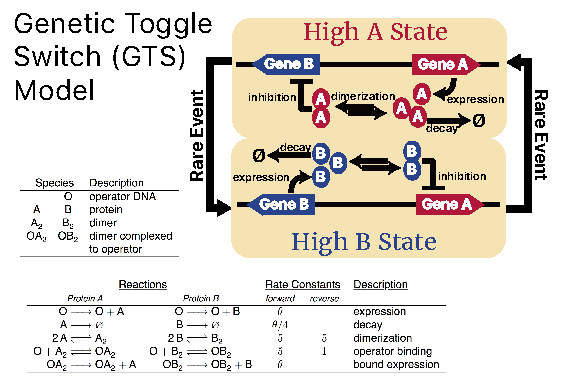
\includegraphics[width=6in]{{../Figures/model_schematics/genetic_toggle_switch}.pdf}
\end{center}

Protein A and protein B are both produced from a single piece of operator DNA. A and B can both dimerize, and each dimer can bind back to the operator DNA. Only one dimer can bind to the DNA at a time. When the DNA is unbound, it will produce both A and B at an equal rate. However, when a dimer of one of the proteins is bound, the DNA will only produce more of that same protein. This means that \abr{GTS} spends the vast majority of its time in either a high A, low B state (state $\statea$), or a high B, low A state (state $\stateb$).

\abr{SRG} has 1 unique chemical species, and thus a 1D state space. \abr{GTS} has 7 unique species and a 7D state space, and so is inherently a much more complex system to simulate and analyze. In particular, complex sources of error emerge in higher dimensional systems that aren't present in 1D systems like \abr{SRG}. Helpfully, \abr{GTS} has a feature that makes it easy to examine simulation error: it's perfectly symmetric in terms of proteins A and B. In fact, because the species and reactions containing A are identical to those containing B (aside from, of course, the change in protein), the \abr{MFPT} of the $\atob$ transition is equal to that of $\btoa$, and the probability landscape of \abr{GTS} is perfectly symmetrical. The deviation from this 2-fold symmetry can thus be used as a simple measure of simulation accuracy.

Over the course of the previous chapters in this tutorial we established the theory and protocols for running and analyzing FFPilot simulations. In this chapter we'll focus on error, and how to think about simulation accuracy in general.

\section{FFPilot simulation input for GTS}

The protocol for setting up the input for an FFPilot simulation of \abr{GTS} is very similar that used in the earlier chapters for setting up simulations of \abr{SRG}. Essentially, certain array values, such as \code{\oparamcoeffs} and \code{\tilingbasins}, which were 1D for \abr{SRG} are 7D for \abr{GTS}. Although this may sound complex, in practice it is not much more complex than setting up \abr{SRG}.

Once again, we're going to use the \exe{lm_sbml_import} to convert a \path{.sbml} file to an \path{.lm} file, and then use the \code{h5py} Python package to add the needed order parameter and tiling.

First, we run the \exe{lm_sbml_import} utility on \pth{\sbml} in order to produce \pth{\lm}. Open a terminal, then \sh{cd} to \pth{\dir} and then execute:

\inputcmd{snippets/gts/lm_sbml_import.sh}

Next we set the order parameter, the tiling, and the FFPilot simulation options needed for landscape output using the following Python scripts:\\
\\
\textbf{order parameter}

\inputpy{snippets/gts/add_order_parameter.py}

\textbf{tiling}

\inputpy{snippets/gts/add_tiling.py}

\textbf{FFPilot simulation options}

\inputpy{snippets/gts/add_options.py}

\section{Running the simulation}
No surprises here, as the \abr{GTS} simulation can be executed with the same basic command that was used to run the \abr{SRG} simulations:

\inputcmd{snippets/gts/lmes.sh}

\section{MFPT to each edge of GTS tiling}

As with our \abr{SRG} simulations, the \abr{MFPT} values of \abr{GTS} can be fetched directly from the simulation stage summary records. Follow the instructions given in \secref{sec:fetch_mfpt_srg} in order to retrieve the \abr{MFPT} results from the \abr{GTS} simulation we just ran. Plotting those values should yield something along the lines of:
 
\begin{center}
    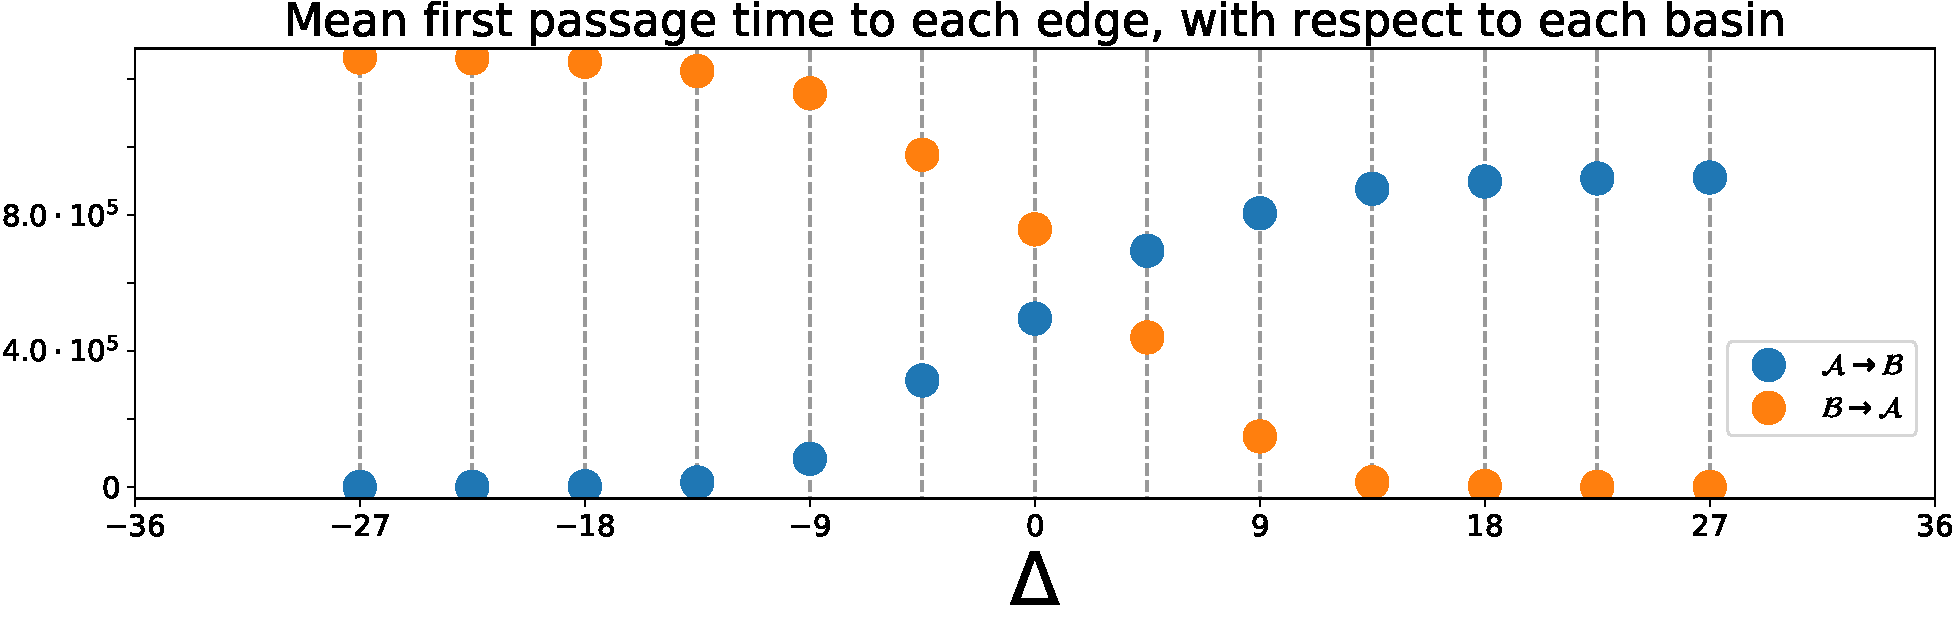
\includegraphics[width=6.0in]{{../Figures/gts_edge_mfpt}.pdf}
\end{center}

There are two sets of GTS MFPT values, those collected when switching $\atob$ and when switching $\btoa$. Regardless of what kind of simulation was used to estimate them, they should be perfectly symmetrical. This means that if one set is flipped with respect to its edges, the two sets would then be equal. However, complete equality is unlikely to be observed in the results from a 10\% error goal simulation. Instead, it is far more likely that some deviation between the two sets of MFPTs will occur:

\begin{center}
    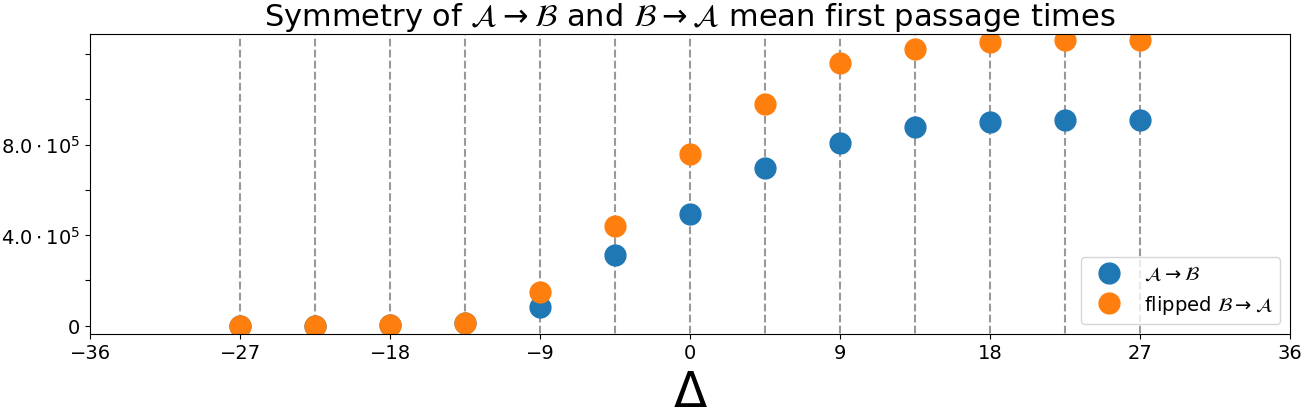
\includegraphics[width=6.0in]{{../Figures/gts_edge_mfpt_symmetry}.pdf}
\end{center}

When GTS is simulated using a 1\% error goal, much less deviation occurs between the results from the $\atob$ and $\btoa$ processes:

\begin{center}
    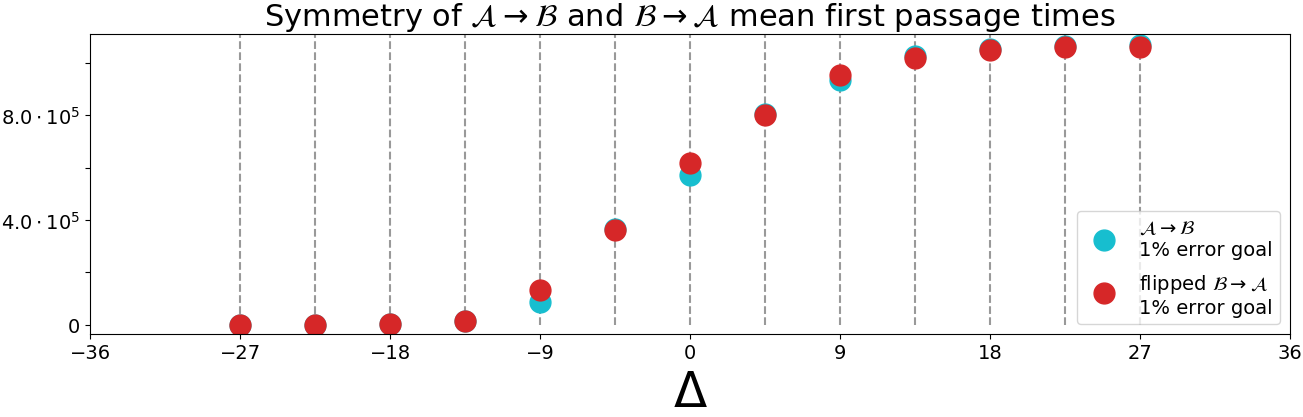
\includegraphics[width=6.0in]{{../Figures/gts_edge_mfpt_symmetry_err_01}.pdf}
\end{center}

As can be seen above, even though some deviations do begin to develop in phases immediately before or around the transition midpoint (\ie $\Delta = 0$), the simulation recovers from those deviations, and they do not persist into the overall basin-to-basin \abr{MFPT} estimates. This can be though of as a signature of the technique which FFPilot uses to optimize computational efficiency. The optimizing equation that drives FFPilot tends to bias simulations against running too many trajectories during the most expensive phases (for \abr{GTS}, the most expensive phases are indeed those in the vicinity of the transition midpoint), and makes up for any errors this might introduce by causing more simulations to be run during the least expensive phases.

\section{Landscape of the transition region}
The code we introduced last chapter in \secref{sec:landscape_srg} for calculating the landscape of \abr{SRG} is flexible enough to be reused almost in its entirety when calculating the landscape of the very different \abr{GTS}. The only major differences are that we will use the \abr{GTS} specific 1D order parameter $\oparamd$, and also define a 2D order parameter $\oparamab$ to do some fancy plotting with:

\inputpy{snippets/gts/order_parameter_functions.py}

\subsection{Calculating the transition region landscape}

The code from \secref{sec:srg_stage_hists} can be used to produce the \abr{GTS} stage histograms:

\begin{center}
    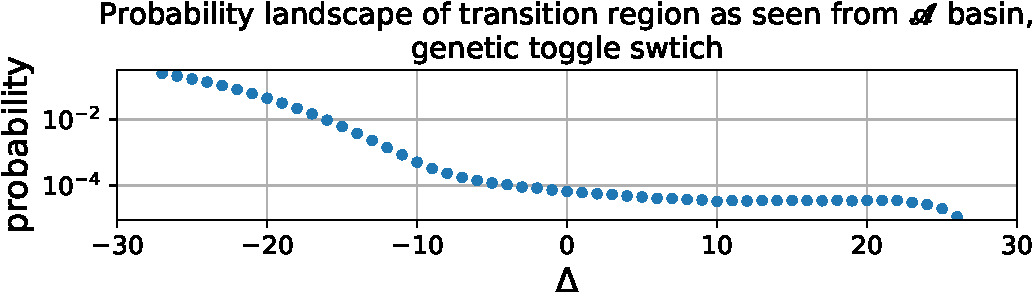
\includegraphics[width=6.0in]{{../Figures/gts_landscape_0_basin}.pdf}
\end{center}
\begin{center}
    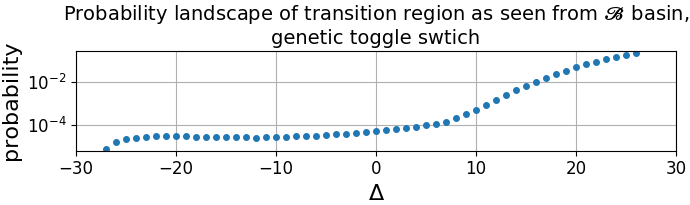
\includegraphics[width=6.0in]{{../Figures/gts_landscape_1_basin}.pdf}
\end{center}

The \abr{GTS} stage histograms can then be combined into a single transition region landscape using the code from \secref{sec:srg_transition_landscape}:

\begin{center}
    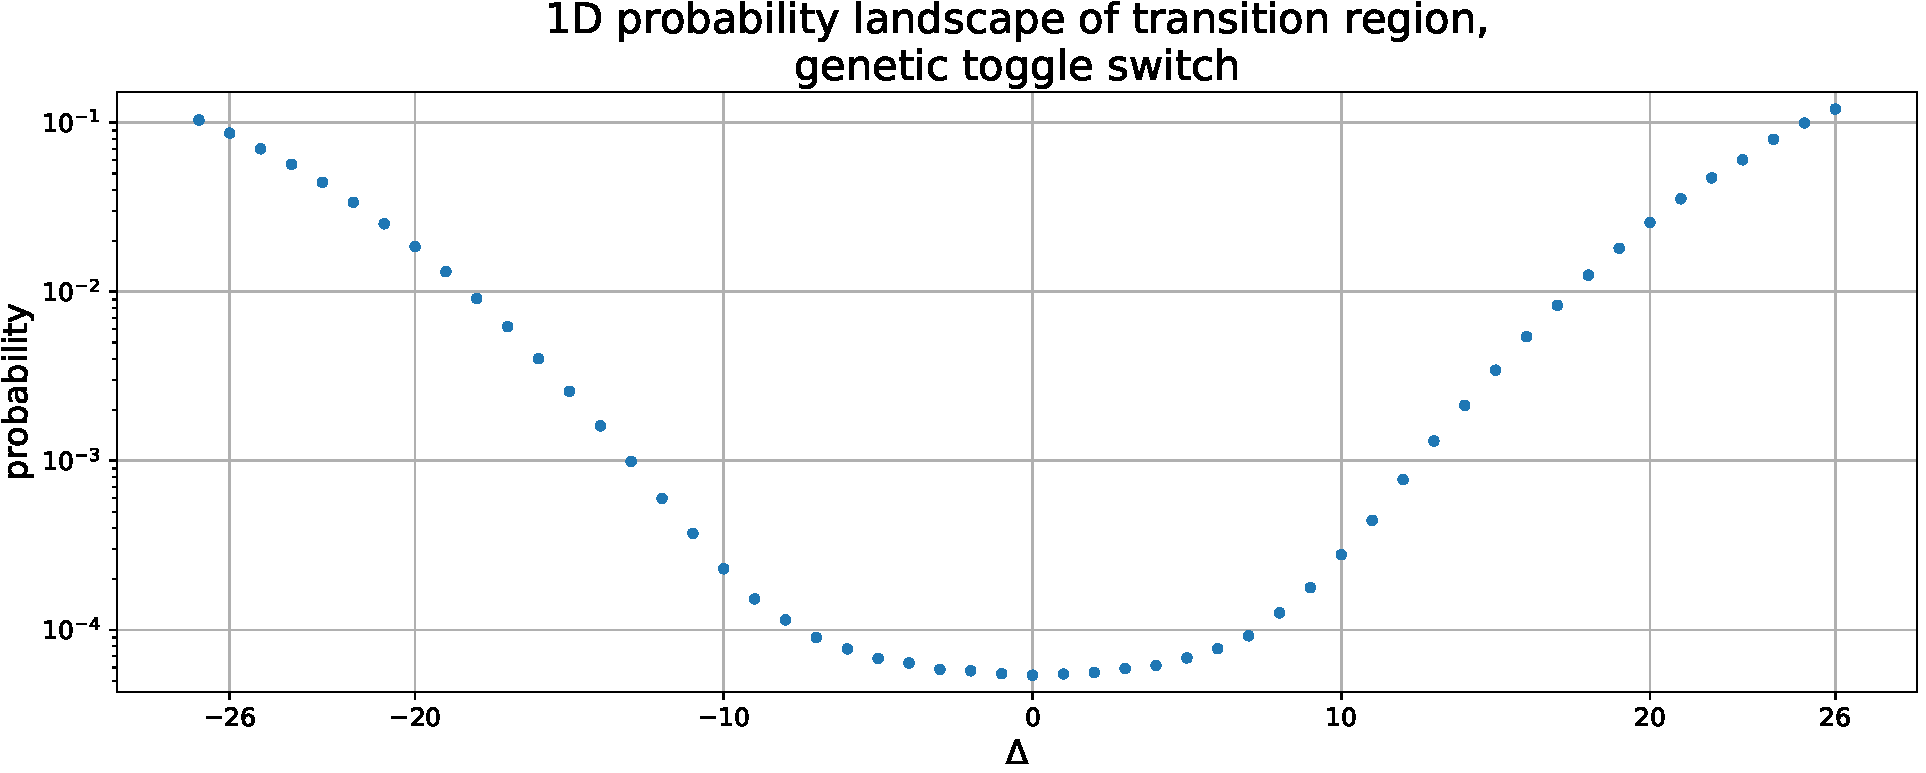
\includegraphics[width=6.0in]{{../Figures/gts_landscape_transition_1d}.pdf}
\end{center}

A great deal more detail can be gleaned when the transition is plotted using the 2D $\oparamab$ order parameter:

\begin{center}
    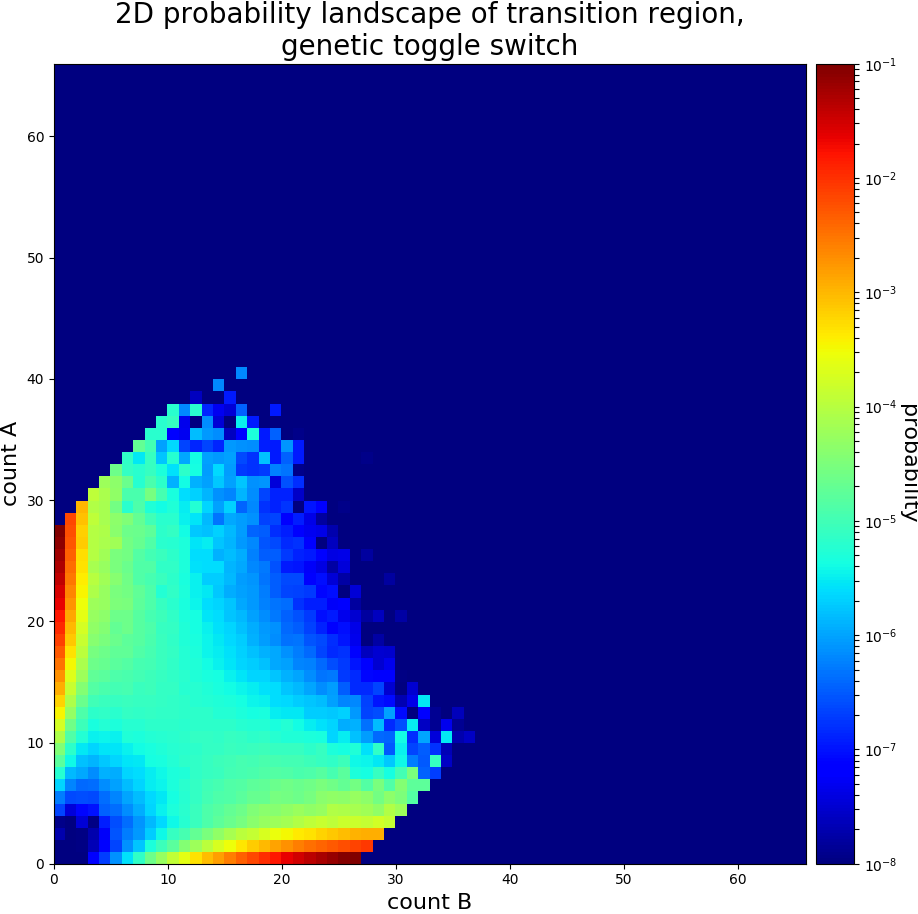
\includegraphics[width=6.0in]{{../Figures/gts_landscape_transition_2d}.pdf}
\end{center}

\subsection{Accuracy of the calculated transition region landscape}

In terms of the 1D order parameter $\Delta$ (ie $\text{count A} - \text{count B}$), the GTS landscape is symmetric over the origin. In terms of the 2D order parameter $\{\text{count A}, \text{count B}\}$, GTS is symmetric over the line $x=y$. These symmetries are important, since they offer a simple way to test the accuracy of our landscape assembly procedure (which includes both the simulation and the analysis). For any landscape we calculate, the closer its two halves are to perfect symmetry the more accurate the assembly procedure was.

Symmetry, or lack thereof, is usually easier to spot in plots of 1D order parameters. Though somewhat analytically crude, a comparison of any two symmetric points ${-x, x}$ in the landscape can be used as a simple, quantitative measure of the landscape's overall accuracy. A sense of how FFPilot error goal affects the accuracy of the landscape can be gained by comparing the two symmetric points $\Delta=-26$ and $\Delta=26$. When a landscape is calculated from a 10\% error goal FFPilot simulation, the divergence between the probabilities of -26 and 26 tends to be quite large, on the order of $10-20\%$:

\begin{center}
    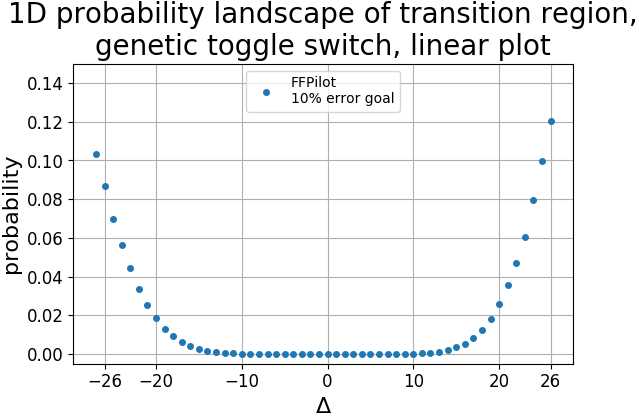
\includegraphics[width=6.0in]{{../Figures/gts_landscape_transition_1d_linear}.pdf}
\end{center}

 On the other hand, as in the plot shown below, the probabilities of -26 and 26 are nearly equal when calculated using data from a 1\% error goal simulation:

\begin{center}
    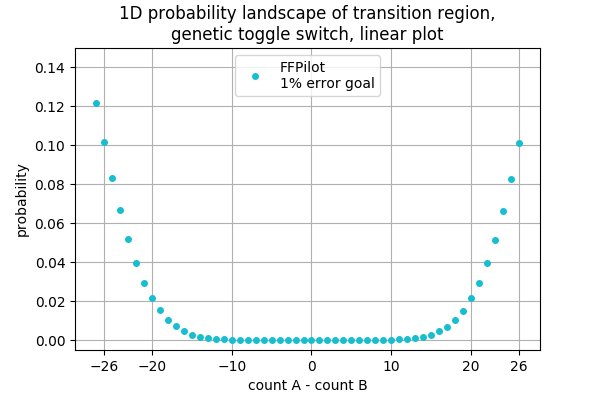
\includegraphics[width=6.0in]{{../Figures/gts_transition_1d_err_01}.pdf}
\end{center}

The landscape shown above was produced from the example data included with the notebook (in the \pth{example_arrays/landscape_ffpilot_basin_\%d.npz} files).

\section{The complete unbiased landscape of GTS}

\subsection{Calculating the complete landscape}
Now that we have the transition landscape assembled, the complete landscape can be calculated by simply reusing the code from \secref{sec:srg_complete_landscape}. Plotted in 1D (along the $\oparamd$ order parameter) and 2D (along the $\oparamab$ order parameter) it looks like:

\begin{center}
    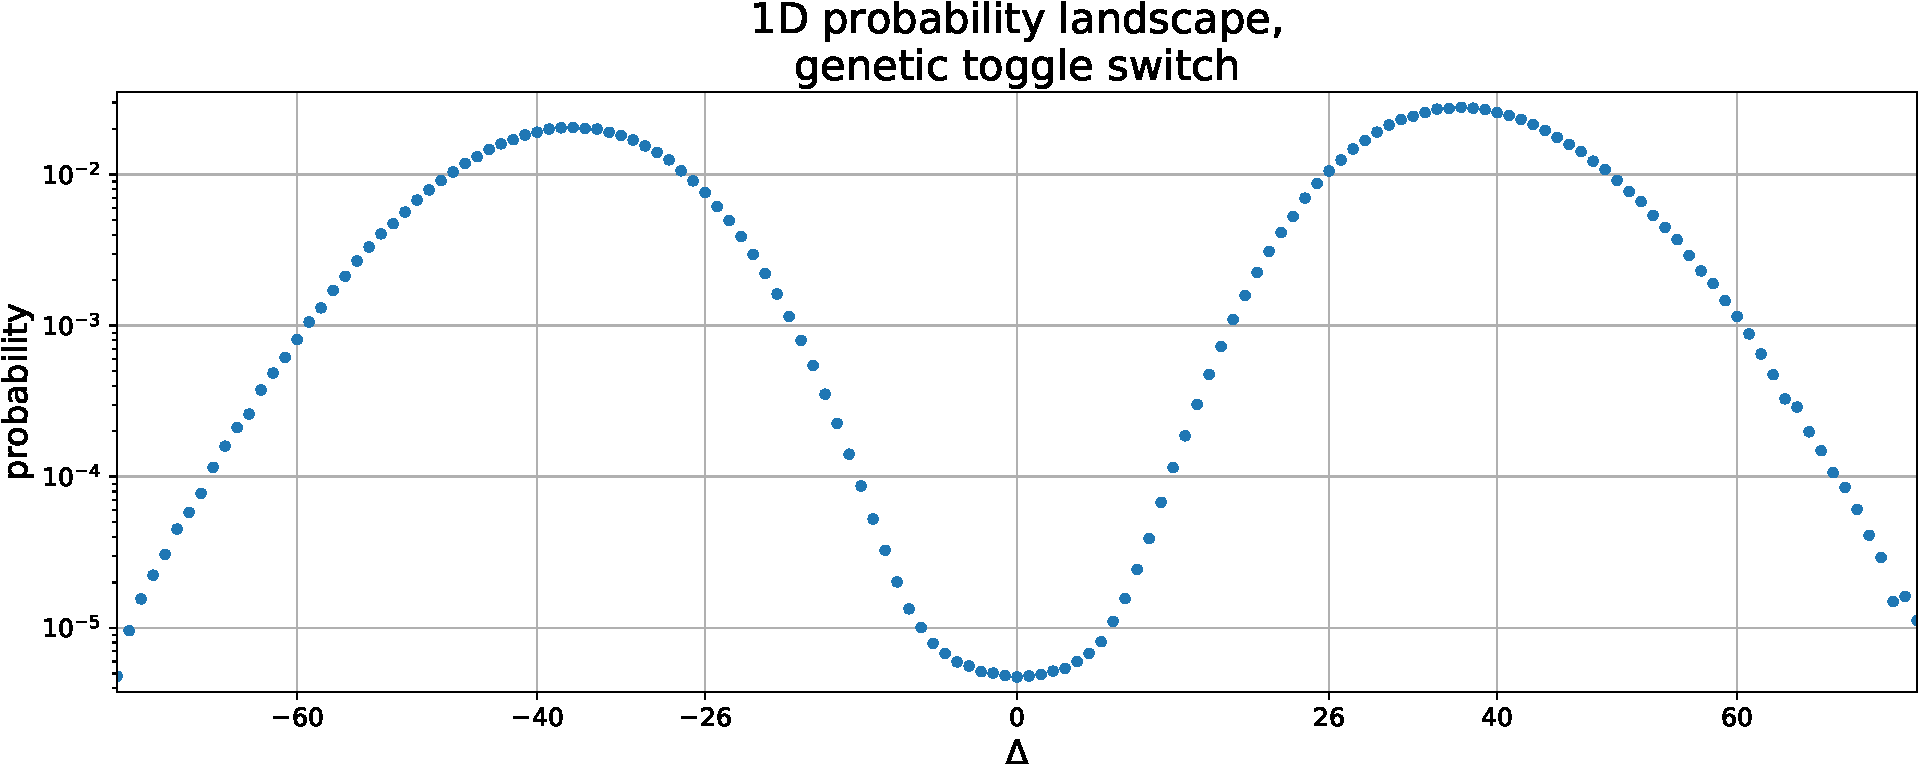
\includegraphics[width=6.0in]{{../Figures/gts_landscape_1d}.pdf}
\end{center}

\begin{center}
    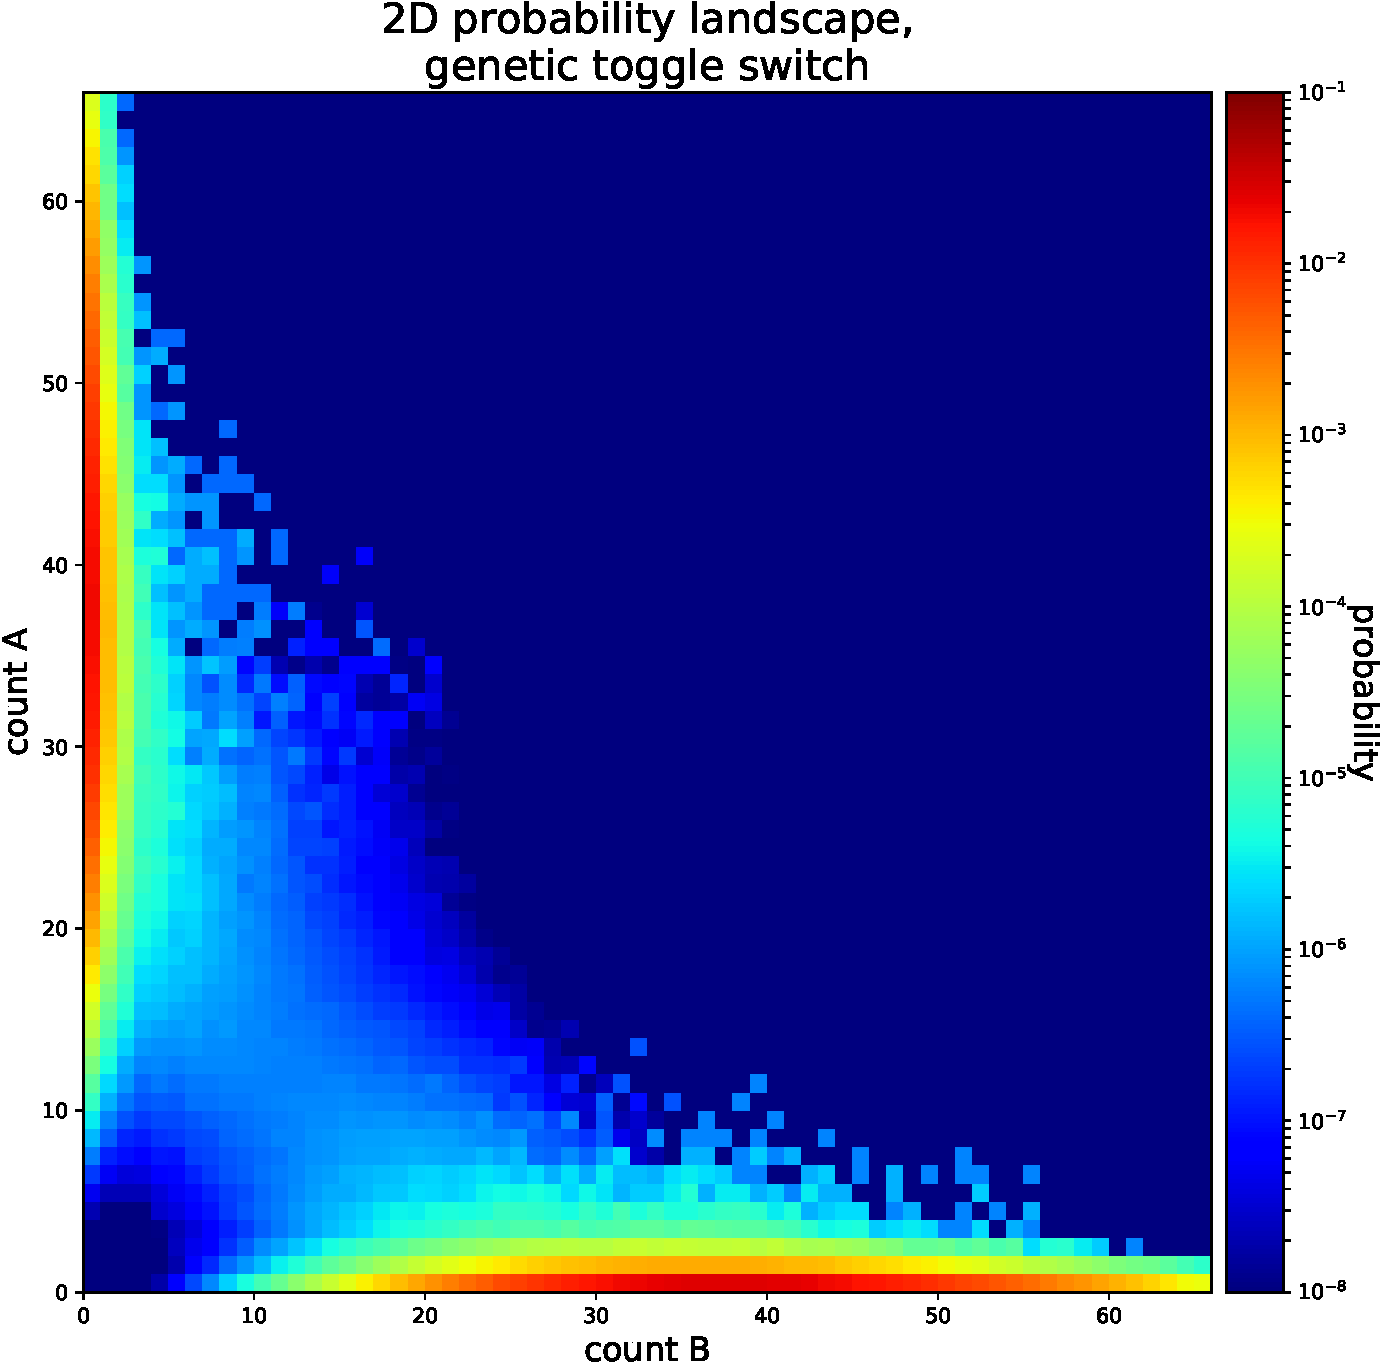
\includegraphics[width=6.0in]{{../Figures/gts_landscape_2d}.pdf}
\end{center}

As you can see above, the fitting procedure in the code we wrote last chapter is robust and flexible enough that it is able to deal with both the \abr{SRG} and the (very much different) \abr{GTS} models.

\subsection{Accuracy of calculated complete landscape: comparison with replicate sampling}
In addition to comparing them against each other, we can also gauge the accuracy of the  two halves of a \abr{GTS} FFPilot simulation by comparing them to the results from a \abr{DS} simulation. Though \abr{DS} simulation is computationally inefficient, it is highly accurate. It has been shown\cite{Gillespie:2007bx} that \abr{DS} simulation will converge roughly monotonically to the correct answer under a large variety of conditions. This convergence behavior, along with a history of decades of use and verification, allows \abr{DS} results to be used as a sort of gold standard when examining novel simulation methods. Here is a comparison of the transition region calculated by FFPilot and \abr{DS} simulations:

\begin{center}
    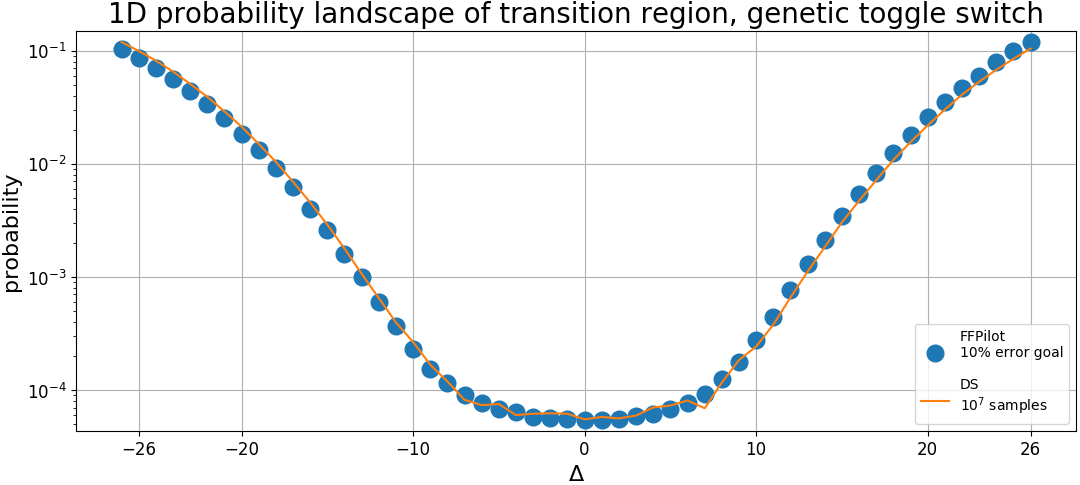
\includegraphics[width=6.0in]{{../Figures/gts_landscape_transition_vs_bf}.pdf}
\end{center}

The landscape produced by FFPilot is much less noisy than the landscape from direct sampling in the immediate neighborhood of the transition point. In terms of landscapes, FFPilot simulation is at its most useful in any region of extremely low probability. Direct sampling tends to struggle with these low probability regions, and can only collect enough samples to map their landscapes with reasonable accuracy when vast computational resources are used.

This version of the genetic toggle switch is completely symmetric in terms of A and B. Thus, the two peaks in the probability distribution should be the same height. The peak on the left corresponds to state $\mathcal{A}$ (in which there is a high count of protein A and a low count of protein B) and the peek on the right corresponds to state $\mathcal{B}$ (in which there is a high count of protein B and a low count of protein A). In terms of the 1D $\oparamd$, the two peeks $\mathcal{A}$ and $\mathcal{B}$ fall at -37 and 37, respectively.

\begin{center}
    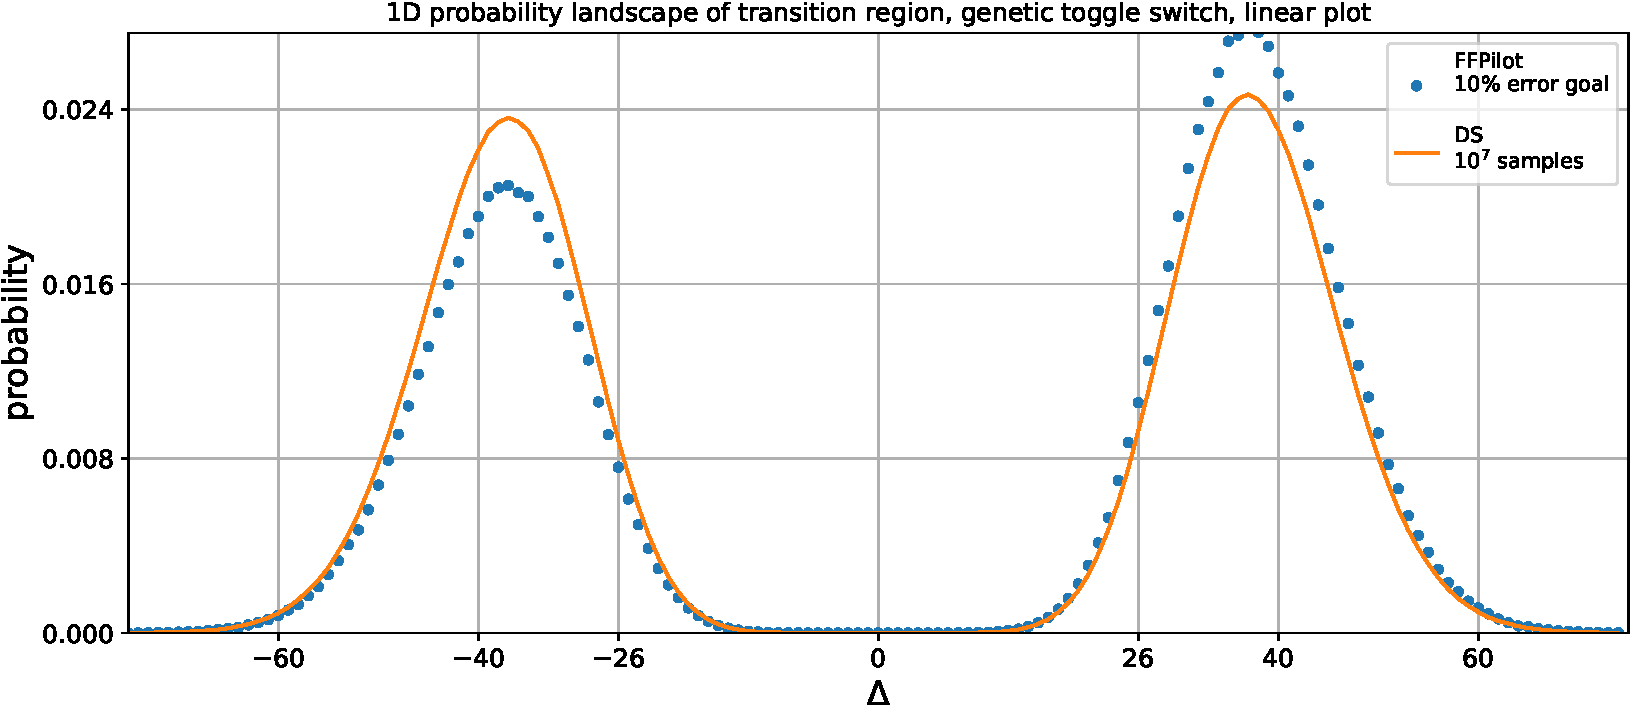
\includegraphics[width=6.0in]{{../Figures/gts_landscape_vs_bf_linear}.pdf}
\end{center}

In the direct sampling data we show above, the height of the state $\mathcal{A}$ and state $\mathcal{B}$ peeks differ by about ${\sim}4.5\%$ relative to one another. Whether FFPilot under- or out-performs this figure depends on the error goal with which a simulation is run. Error goal is expressed in terms of a desired level of error in the estimated MFPT from a simulation, but a lower error goal also tends to reduce error in other measures as well, including this landscape symmetry measure.

In landscapes produced from FFPilot simulations run at an error goal of 10\%, the two peeks can differ by 10\% or more. However, the difference in the peeks decreases dramatically for FFPilot simulations run with a 1\% error goal. The landscape shown below was produced from the example data included with the notebook (in the \\
\code{data_example/landscape_ffpilot_basin_\%d.npz} files), which was obtained from an FFPilot simulation run with a 1\% error goal:

\begin{center}
    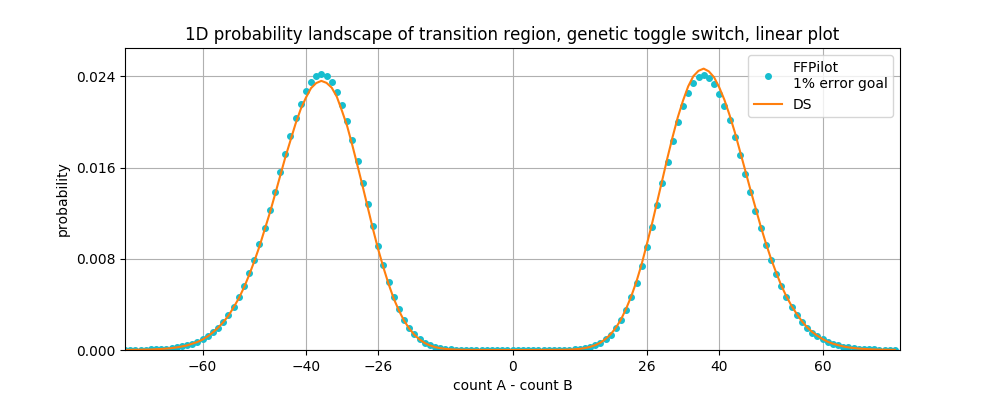
\includegraphics[width=6.0in]{{../Figures/gts_land_1d_err_01_linear}.pdf}
\end{center}

In the landscape produced by FFPilot the heights of the $\mathcal{A}$ and $\mathcal{B}$ peeks are closely matched, and differ by less than 0.7\%. In this case FFPilot outperformed direct sampling in terms of correctly reproducing the underlying symmetry of the genetic toggle switch's landscape.
}
